% !TEX TS-program = XeLaTeX
\documentclass[10pt,handout]{beamer}

\usepackage{ragged2e}
\usepackage{fontspec}
\usepackage{xcolor}
\usepackage{tikz}
\usepackage{listings}
\usepackage{amsmath}
\usepackage{xspace}
\usepackage{adjustbox}
\usepackage{xspace}
\usepackage{fitch}
\usepackage{hyperref}
\usepackage[normalem]{ulem}

\usefonttheme{professionalfonts} % using non standard fonts for beamer
\usefonttheme{serif} % default family is serif
\setmainfont{Helvetica Neue}

\definecolor{cmu_red}{RGB}{153,0,0}					% #990000
\definecolor{cmu_dark_grey}{RGB}{70, 70, 70}		% #464646
\definecolor{cmu_light_grey}{RGB}{212, 212, 212}	% #d4d4d4
\definecolor{cmu_light_tan}{RGB}{243,240,233}		% #f3f0e9
\definecolor{cmu_violet}{RGB}{100,76,86}			% #674c56
\definecolor{cmu_blue}{RGB}{116,147,162}			% #7493a2
\definecolor{cmu_mustard}{RGB}{193,165,98}			% #c1a562
\definecolor{cmu_brown}{RGB}{147,98,65}				% #936241
\definecolor{cmu_orange}{RGB}{209,119,2}			% #d17702
\definecolor{cmu_green}{RGB}{153,153,51}			% #999933
\definecolor{cmu_tan}{RGB}{172,157,116}				% #ac9d74
\definecolor{mygray}{rgb}{0.5,0.5,0.5}

\mode<presentation>{
	\usetheme{Berlin}
	\usecolortheme{beaver}
} 

\setbeamercolor{title}{fg=white,bg=cmu_red}
\setbeamercolor{frametitle}{bg=cmu_red,fg=white}
\setbeamercolor{itemize item}{bg=white,fg=black}
\setbeamercolor{enumerate item}{bg=white,fg=black}
\setbeamercolor{enumerate subitem}{bg=white,fg=black}

\setbeamertemplate{headline}{}
\setbeamertemplate{itemize items}[default]
\setbeamertemplate{enumerate items}[default]

\usenavigationsymbolstemplate{}

\makeatletter
\defbeamertemplate*{footline}{myfootline}
{
  \leavevmode%
  \hbox{%
  \begin{beamercolorbox}[wd=.333333\paperwidth,ht=2.25ex,dp=1ex,center]{title in head/foot}%
    \usebeamerfont{author in head/foot}\insertshortauthor\expandafter\beamer@ifempty\expandafter{\beamer@shortinstitute}{}{~~\insertshortinstitute}
  \end{beamercolorbox}%  
  \begin{beamercolorbox}[wd=.333333\paperwidth,ht=2.25ex,dp=1ex,center]{title in head/foot}%
    \usebeamerfont{title in head/foot}\insertshorttitle
  \end{beamercolorbox}%
  \begin{beamercolorbox}[wd=.333333\paperwidth,ht=2.25ex,dp=1ex,right]{title in head/foot}%
    % \usebeamerfont{date in head/foot}\insertshortdate{}\hspace*{2em}
    \insertframenumber{} / \inserttotalframenumber\hspace*{2ex} 
  \end{beamercolorbox}}%
  \vskip0pt%
}
\makeatother
\setbeamertemplate{footline}[myfootline]

\lstdefinestyle{customc}{
  belowcaptionskip=1\baselineskip,
  breaklines=true,
  language=C,
  showstringspaces=false,
  numbers=none,
  % xleftmargin=1ex,
  framexleftmargin=1ex,
  % numbersep=5pt,
  % numberstyle=\tiny\color{mygray},
  basicstyle=\footnotesize\ttfamily,
  keywordstyle=\color{blue},
  commentstyle=\itshape\color{purple!40!black},  
  stringstyle=\color{orange},
  morekeywords={output,assume,observe,input,bool,then,fun,match,in,val,list,type,of,string,unit,let,bytes,mov,imul,add,sar,shr,function,forall,nat,requires,ensures,method,returns,assert,new,array,modifies,reads,old,predicate,lemma,seq,calc,nan,var},
  tabsize=2,
  deletestring=[b]',
  backgroundcolor=\color{gray!15},
  frame=tb
}
\lstset{escapechar=@,style=customc}

\NewDocumentCommand{\redcallout}{r<> O{text opacity=1} m m}{%
\tikz[remember picture, overlay]\node[align=center,fill=red!65!black,#2,visible on=<#1>,rounded corners,rectangle callout,anchor=pointer,callout relative pointer={(230:1cm)},text=white,minimum width=4cm,inner sep=5pt]
at (#3) {#4};
}

\NewDocumentCommand{\redcalloutpos}{r<> O{text opacity=1} m m m}{%
\tikz[remember picture, overlay]\node[align=center,fill=red!65!black,#2,visible on=<#1>,rounded corners,rectangle callout,anchor=pointer,callout relative pointer={(#5:1cm)},text=white,minimum width=4cm,inner sep=5pt]
at (#3) {#4};
}

\newcommand{\tikzmark}[1]{\tikz[overlay,remember picture,xshift=-0.9ex] \node (#1) {};}

\newcommand{\nondeterm}{\xspace\ensuremath{[]}\xspace}

\tikzstyle{database}=
[
  cylinder,
  shape border rotate=90,
  aspect=0.25,
  draw,
  thick,
  text width=10ex,
  minimum width=10ex,
  align=center,
  minimum height=4.5em
]
\tikzstyle{process}=
[
  rounded corners=3pt,
  draw,
  thick,
  text width=9ex,
  minimum width=10ex,
  align=center,
  minimum height=4.5em
]
\tikzstyle{result}=
[
  rounded rectangle,
  draw,
  thick,
  text width=9ex,
  align=center,
  minimum height=2em
]
\tikzstyle{blockarrow}=
[
  draw,
  thick,
  ->
]

\tikzset{
  treenode/.style = {align=center},
  root/.style     = {treenode, font=\footnotesize},
  env/.style      = {treenode, font=\footnotesize},
  dummy/.style    = {treenode}
}

\definecolor{mygray}{rgb}{0.5,0.5,0.5}
\definecolor{backgray}{gray}{0.95}
\lstdefinestyle{customjava}{
  belowcaptionskip=1\baselineskip,
  breaklines=true,
  language=C,
  showstringspaces=false,
  numbers=left,
  xleftmargin=2em,
  framexleftmargin=1.5em,
  numbersep=5pt,
  numberstyle=\tiny\color{mygray},
  basicstyle=\footnotesize\ttfamily,
  keywordstyle=\color{blue},
  commentstyle=\itshape\color{purple!40!black},
  tabsize=2,
  backgroundcolor=\color{backgray},
  escapechar=\%
}

\usetikzlibrary{automata,shapes,positioning,matrix,shapes.callouts,decorations.text,arrows}

\tikzset{onslide/.code args={<#1>#2}{%
  \only<#1>{\pgfkeysalso{#2}} % \pgfkeysalso doesn't change the path
}}

\tikzset{
    invisible/.style={opacity=0,text opacity=0},
    visible on/.style={alt={#1{}{invisible}}},
    alt/.code args={<#1>#2#3}{%
      \alt<#1>{\pgfkeysalso{#2}}{\pgfkeysalso{#3}} % \pgfkeysalso doesn't change the path
    },
  }

\newcommand{\true}{\ensuremath{\mathit{true}}\xspace}
\newcommand{\false}{\ensuremath{\mathit{false}}\xspace}

\title[Software Foundations of S \& P]{
\RaggedRight
	Software Foundations of Security \& Privacy \\
	\ 15316 Spring 2018 \\
	\ Lecture 1: \\
	\ Introduction
}

\author[Matt Fredrikson]{
	Matt Fredrikson \\
	mfredrik@cs
}

\begin{document}
\setlength\abovedisplayskip{5pt}
\setlength\belowdisplayskip{5pt}

%%%%%%%%%%%%%%%%%%%%%%%%%%%%%%

\begin{frame}
\titlepage
\end{frame}

%%%%%%%%%%%%%%%%%%%%%%%%%%%%%%

\begin{frame}

\frametitle{Course Staff}

\begin{columns}

\begin{column}{0.5\textwidth}
\centering
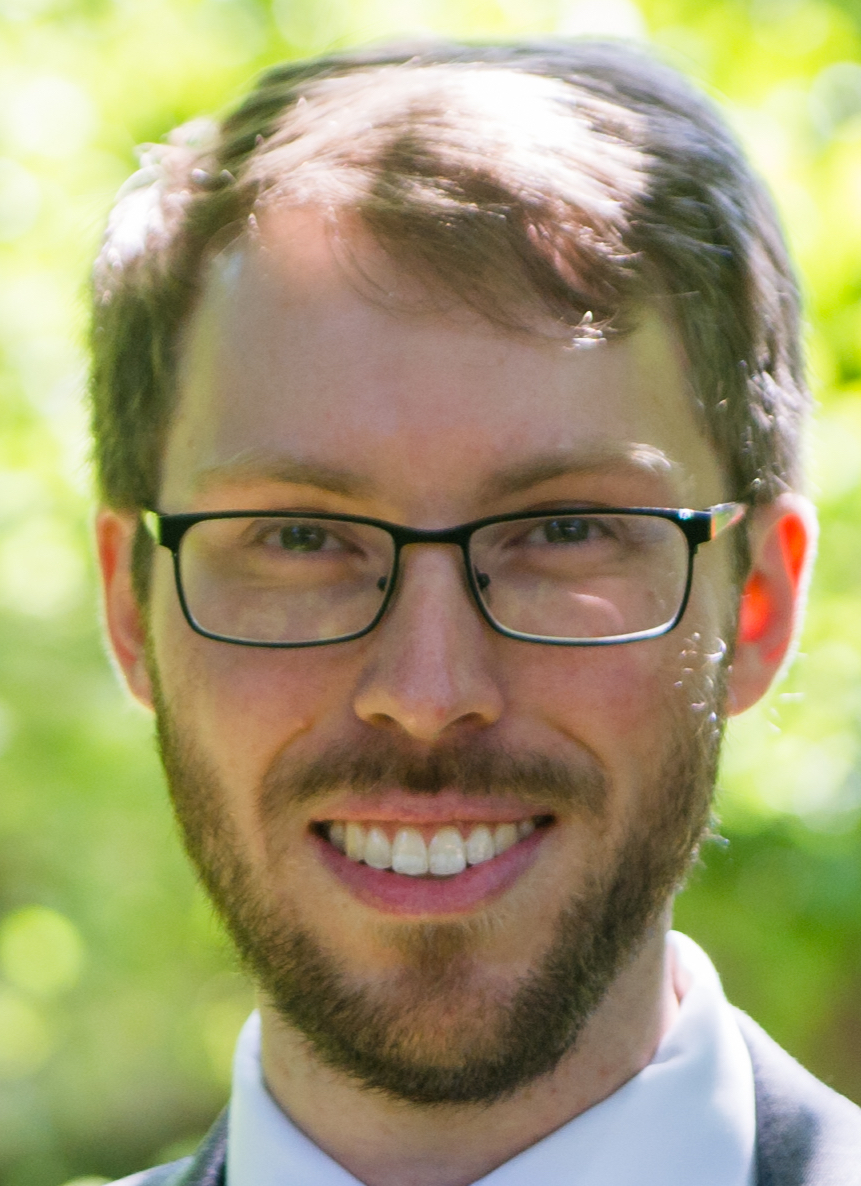
\includegraphics[height=8em]{matt.jpg}

Matt Fredrikson \\
Instructor
\end{column}

\begin{column}{0.5\textwidth}
\centering
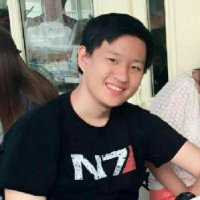
\includegraphics[height=8em]{tianyu.jpg}

Tianyu Li \\
TA
\end{column}

\end{columns}

\end{frame}

%%%%%%%%%%%%%%%%%%%%%%%%%%%%%%

\begin{frame}

\frametitle{Recent news...}

\centering
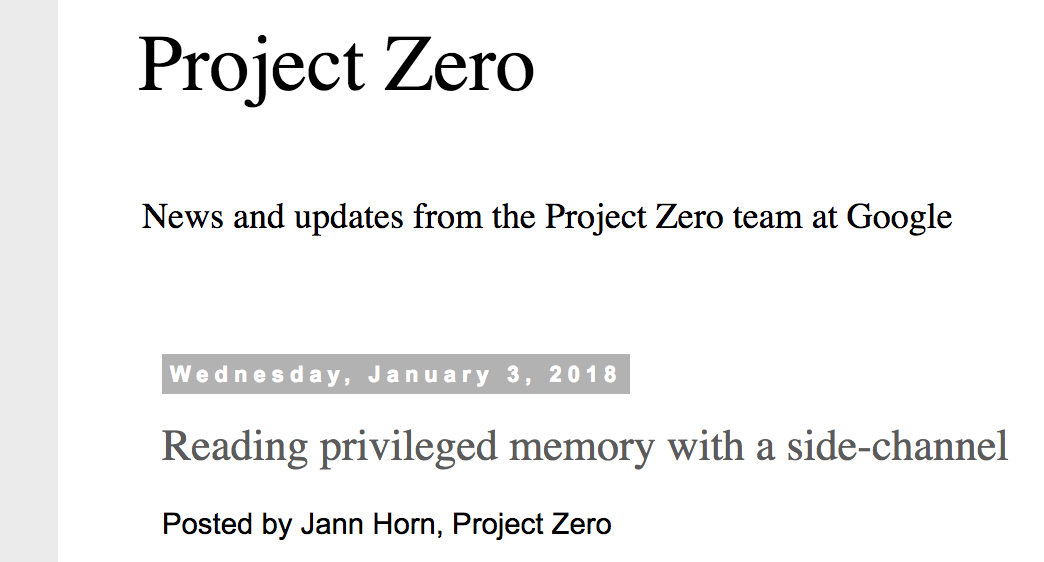
\includegraphics[height=15em]{sidechan-blog.png}

\end{frame}

%%%%%%%%%%%%%%%%%%%%%%%%%%%%%%

\begin{frame}

\frametitle{Spectre \& Meltdown}

What's the big deal? \pause
\begin{itemize}
\item ``Efficiently'' leak information via mis-speculated execution
\item Read arbitrary virtual memory regions (including kernel)
\item Bypass explicit bounds checks
\item Violate browser sandboxing
\item ...? \\[1em]
\end{itemize}

\pause
\begin{center}
``Every Intel processor that implements out-of-order execution is potentially affected''
\\[1ex] \pause
... \emph{which is effectively every processor since 1995}.
\end{center}

\end{frame}

%%%%%%%%%%%%%%%%%%%%%%%%%%%%%%

\begin{frame}[fragile]

\frametitle{Timing channels}

\begin{lstlisting}[basicstyle=\small,style=customjava]
struct array {
 unsigned long length;
 unsigned char data[];
};
struct array *arr1 = ...; /* small array */
struct array *arr2 = ...; /* array of size 0x400 */
unsigned long untrusted_offset = network_read(...);
unsigned char value = arr1->data[untrusted_offset];
unsigned long index2 = ((value&1)*0x100)+0x200;
unsigned char value2 = arr2->data[index2];
\end{lstlisting}

\end{frame}

%%%%%%%%%%%%%%%%%%%%%%%%%%%%%%

\begin{frame}[fragile]

\frametitle{Timing channels}

\begin{lstlisting}[basicstyle=\small,style=customjava]
struct array {
 unsigned long length;
 unsigned char data[];
};
struct array *arr1 = ...; /* small array */
struct array *arr2 = ...; /* array of size 0x400 */
%\color{red}{\small unsigned long untrusted\_offset = network\_read(...);}%
%\color{red}{\small unsigned char value = arr1->data[untrusted\_offset];}%
unsigned long index2 = ((value&1)*0x100)+0x200;
unsigned char value2 = arr2->data[index2];
\end{lstlisting}

\begin{center}
Step 1. Read some data from an arbitrary memory location
\end{center}

\end{frame}

%%%%%%%%%%%%%%%%%%%%%%%%%%%%%%

\begin{frame}[fragile]

\frametitle{Timing channels}

\begin{lstlisting}[basicstyle=\small,style=customjava]
struct array {
 unsigned long length;
 unsigned char data[];
};
struct array *arr1 = ...; /* small array */
struct array *arr2 = ...; /* array of size 0x400 */
unsigned long untrusted_offset = network_read(...);
unsigned char value = arr1->data[untrusted_offset];
%\color{red}{\small unsigned long index2 = ((value\&1)*0x100)+0x200;}%
unsigned char value2 = arr2->data[index2];
\end{lstlisting}

\begin{center}
Step 2. Isolate a bit of data from the read \pause
\begin{itemize}
\item \texttt{index2} is \texttt{0x200} if bit is 0
\item Otherwise, \texttt{index2} is \texttt{0x300}
\end{itemize}
\end{center}

\end{frame}

%%%%%%%%%%%%%%%%%%%%%%%%%%%%%%

\begin{frame}[fragile]

\frametitle{Timing channels}

\begin{lstlisting}[basicstyle=\small,style=customjava]
struct array {
 unsigned long length;
 unsigned char data[];
};
struct array *arr1 = ...; /* small array */
struct array *arr2 = ...; /* array of size 0x400 */
unsigned long untrusted_offset = network_read(...);
unsigned char value = arr1->data[untrusted_offset];
unsigned long index2 = ((value&1)*0x100)+0x200;
%\color{red}{\small unsigned char value2 = arr2->data[index2];}%
\end{lstlisting}

\begin{center}
Step 3. Read from a location dependent on extracted bit
\end{center}

\end{frame}

%%%%%%%%%%%%%%%%%%%%%%%%%%%%%%

\begin{frame}[fragile]

\frametitle{Timing channels}

\begin{lstlisting}[basicstyle=\small,style=customjava]
struct array {
 unsigned long length;
 unsigned char data[];
};
struct array *arr1 = ...; /* small array */
struct array *arr2 = ...; /* array of size 0x400 */
unsigned long untrusted_offset = network_read(...);
unsigned char value = arr1->data[untrusted_offset];
unsigned long index2 = ((value&1)*0x100)+0x200;
unsigned char value2 = arr2->data[index2];
\end{lstlisting}

\begin{center}
Step 4. Time reads to \texttt{arr2->data[0x200]}, \texttt{arr2->data[0x300]}
\pause
\begin{itemize}
\item If \texttt{0x200} takes less time, then extracted bit was 0
\item Otherwise, the extracted bit was 1 \\[1em]
\end{itemize}
\pause
This last step is a result of the processor's data cache!
\end{center}

\end{frame}

%%%%%%%%%%%%%%%%%%%%%%%%%%%%%%

\begin{frame}

\frametitle{Progress}

At this point, the attacker has accomplished:
\begin{enumerate}
  \item Read an arbitrary bit of memory
  \item Exfiltrate value of bit by timing cache hits \& misses \\[1em]
\end{enumerate}\pause

Keeping track of necessary assumptions:
\begin{enumerate}
  \item Process code doesn't check bounds on memory access
  \item Process code is vulnerable to cache side channel
  \item Attacker controls \texttt{untrusted\_offset}
  \item Targeted memory location won't cause segfault
\end{enumerate}

\end{frame}

%%%%%%%%%%%%%%%%%%%%%%%%%%%%%%

\begin{frame}[fragile]

\frametitle{Defensive programming: bounds checks}

\begin{lstlisting}[basicstyle=\small,style=customjava]
struct array {
 unsigned long length;
 unsigned char data[];
};
struct array *arr1 = ...; /* small array */
struct array *arr2 = ...; /* array of size 0x400 */
unsigned long untrusted_offset = network_read(...);
%\color{red}{\small if (untrusted\_offset < arr1->length) \{}%
 unsigned char value = arr1->data[untrusted_offset];
 unsigned long index2 = ((value&1)*0x100)+0x200;
 %\color{red}{\small if (index2 < arr2->length) \{}%
   unsigned char value2 = arr2->data[index2];
 %\color{red}{\small \}}%
%\color{red}{\small \}}%
\end{lstlisting}

\end{frame}

%%%%%%%%%%%%%%%%%%%%%%%%%%%%%%

\begin{frame}[fragile]

\frametitle{Speculative execution}

\begin{lstlisting}[basicstyle=\small,style=customjava]
struct array {
 unsigned long length;
 unsigned char data[];
};
struct array *arr1 = ...; /* small array */
struct array *arr2 = ...; /* array of size 0x400 */
unsigned long untrusted_offset = network_read(...);
%\color{red}{\small if (untrusted\_offset < arr1->length) \{}%
 unsigned char value = arr1->data[untrusted_offset];
 unsigned long index2 = ((value&1)*0x100)+0x200;
 if (index2 < arr2->length) {
   unsigned char value2 = arr2->data[index2];
 }
}
\end{lstlisting}

\begin{itemize}
\item If \texttt{arr1->length} is not in cache, 100 cycles until it fetches
\pause

\item Processor may begin executing inside branch anyway...
\pause

\item If condition is false, results are essentially rolled back
\pause

\item But not the cache!

\end{itemize}

\end{frame}

%%%%%%%%%%%%%%%%%%%%%%%%%%%%%%

\begin{frame}[fragile]

\frametitle{Speculative cache leaks}

\begin{lstlisting}[basicstyle=\small,style=customjava]
struct array {
 unsigned long length;
 unsigned char data[];
};
struct array *arr1 = ...; /* small array */
struct array *arr2 = ...; /* array of size 0x400 */
unsigned long untrusted_offset = network_read(...);
if (untrusted_offset < arr1->length) {}
 %\color{red}{\small unsigned char value = arr1->data[untrusted\_offset];}%
 unsigned long index2 = ((value&1)*0x100)+0x200;
 if (index2 < arr2->length) {
   %\color{red}{\small unsigned char value2 = arr2->data[index2];}%
 }
}
\end{lstlisting}

\begin{center}
\emph{These attacker-controlled reads make measureable changes to the processor cache!}
\end{center}

\end{frame}

%%%%%%%%%%%%%%%%%%%%%%%%%%%%%%

\begin{frame}

\frametitle{Progress}

At this point, the attacker has accomplished:
\begin{enumerate}
  \item Read an arbitrary bit of memory
  \item Exfiltrate value of bit by timing cache hits \& misses \\[1em]
\end{enumerate}

Keeping track of necessary assumptions:
\begin{enumerate}
  \item \sout{Process code doesn't check bounds on memory access}
  \item \textbf{Process code is vulnerable to cache side channel}
  \item Attacker controls \texttt{untrusted\_offset}
  \item Targeted memory location won't cause segfault
\end{enumerate}

\end{frame}

%%%%%%%%%%%%%%%%%%%%%%%%%%%%%%

\begin{frame}

\frametitle{Berkeley Packet Filter}

Packet filters in Linux, BSD provided by usermode processes \pause
\begin{itemize}
  \item Filters are bytecode-interpreted or JIT-compiled, run \emph{in kernel}
  \item Domain specific language for implementing filters
  \item Filter code can access arrays, do arithmetic, perform tests
  \item Triggered by sending data to associated socket \\[1em]
\end{itemize}

\pause
\begin{center}
\emph{Google's Project Zero team showed how to create JITted BPF bytecode that opens a side-channel vulnerability}
\end{center}
\pause
\begin{itemize}
  \item Upshot: unprivileged processes can read all kernel memory
  \item Proof of concept demonstrated 2000 bytes/second
\end{itemize}

\end{frame}

%%%%%%%%%%%%%%%%%%%%%%%%%%%%%%

\begin{frame}[fragile]

\frametitle{Javascript Interpreters}

\begin{lstlisting}[basicstyle=\small,style=customjava]
if (index < simpleByteArray.length) {
  index = simpleByteArray[index | 0];
  index = (((index * 4096)|0) & (TABLE1_BYTES-1))|0;
  localJunk ^= probeTable[index|0]|0;
}
\end{lstlisting}

\vspace*{1em}
This script causes V8 to JIT-compile vulnerable bytecode
\pause
\begin{itemize}
  % \item ``\texttt{|0}'' operations tell interpreter that results are integers
  % \item \texttt{localJunk} ensures operations aren't optimized out
  \item Leaks to cache-status of \texttt{probeTable[}$n$\texttt{*4096]} for $n\in[0..255]$
  \pause\item Problem: Chrome degrades resolution of JS timer
  \pause\item HTML5 \emph{Web Workers} feature can open new thread, repeatedly decrement shared memory value for precise timing
\end{itemize}

\pause
\begin{center}
\textbf{Upshot:} Untrusted websites can read memory of other sites (passwords, CC \#'s, emails, \ldots), extension data, browser settings, \ldots
\end{center}

\end{frame}

%%%%%%%%%%%%%%%%%%%%%%%%%%%%%%

\begin{frame}

\frametitle{First take-home lesson}

\centering

\includegraphics[width=0.9\textwidth]{unsafe.png}

\end{frame}

%%%%%%%%%%%%%%%%%%%%%%%%%%%%%%

\begin{frame}

\frametitle{Mitigations}

How do we fix it?
\\[1em]

\pause
Good question
\begin{itemize}
\item We probably don't know the full scope of the problem
\item Without hardware changes, no apparent universal fix\\[1em]
\end{itemize}

\pause
But there are software-based mitigations
\begin{enumerate}
  \pause\item Disable speculative execution \pause\emph{(expensive!)}
  \pause\item Disable caching \pause\emph{(probably even more expensive!)}
  \pause\item Selectively disable spec. execution \pause\emph{(hardware changes?)}
  \pause\item \textbf{Never index arrays on untrusted values}
\end{enumerate}

\end{frame}

%%%%%%%%%%%%%%%%%%%%%%%%%%%%%%

\begin{frame}[fragile]

\frametitle{But if you must...}

\begin{lstlisting}[basicstyle=\small,style=customjava]
struct array {
 unsigned long length;
 unsigned char data[];
};
struct array *arr1 = ...; /* 0-padded to size 0xFF */
struct array *arr2 = ...; /* 0-padded size 0xFFF */
unsigned long untrusted_offset = network_read(...);
unsigned char value = arr1->data[untrusted_offset & 0xFF];
unsigned long index2 = ((value&1)*0x100)+0x200;
unsigned char value2 = arr2->data[index2 & 0xFFF];
\end{lstlisting}

\vspace*{1em}
\emph{Only} when you have a good reason to require untrusted indexing,
\begin{itemize}
\pause\item Make sure the target array never contains secrets
\pause\item Pad arrays and implement \emph{logical sandboxing}
\pause\item Use a static checker to make sure you've done this correctly
\end{itemize}

\end{frame}

%%%%%%%%%%%%%%%%%%%%%%%%%%%%%%

\begin{frame}

\frametitle{Mitigations}

How do we fix it?
\\[1em]

Good question
\begin{itemize}
\item We probably don't know the full scope of the problem
\item Without hardware changes, no apparent universal fix\\[1em]
\end{itemize}

But there are software-based mitigations
\begin{enumerate}
  \item Disable speculative execution \emph{(expensive!)}
  \item Disable caching \emph{(probably even more expensive!)}
  \item Selectively disable spec. execution \emph{(hardware changes?)}
  \item \textbf{Never index arrays on untrusted values}
  \pause \item \textbf{Check untrusted code for side channels} \pause \emph{(sounds hard?)}
\end{enumerate}

\end{frame}

%%%%%%%%%%%%%%%%%%%%%%%%%%%%%%

\begin{frame}

\frametitle{Ongoing research: provable side-channel security}

\centering
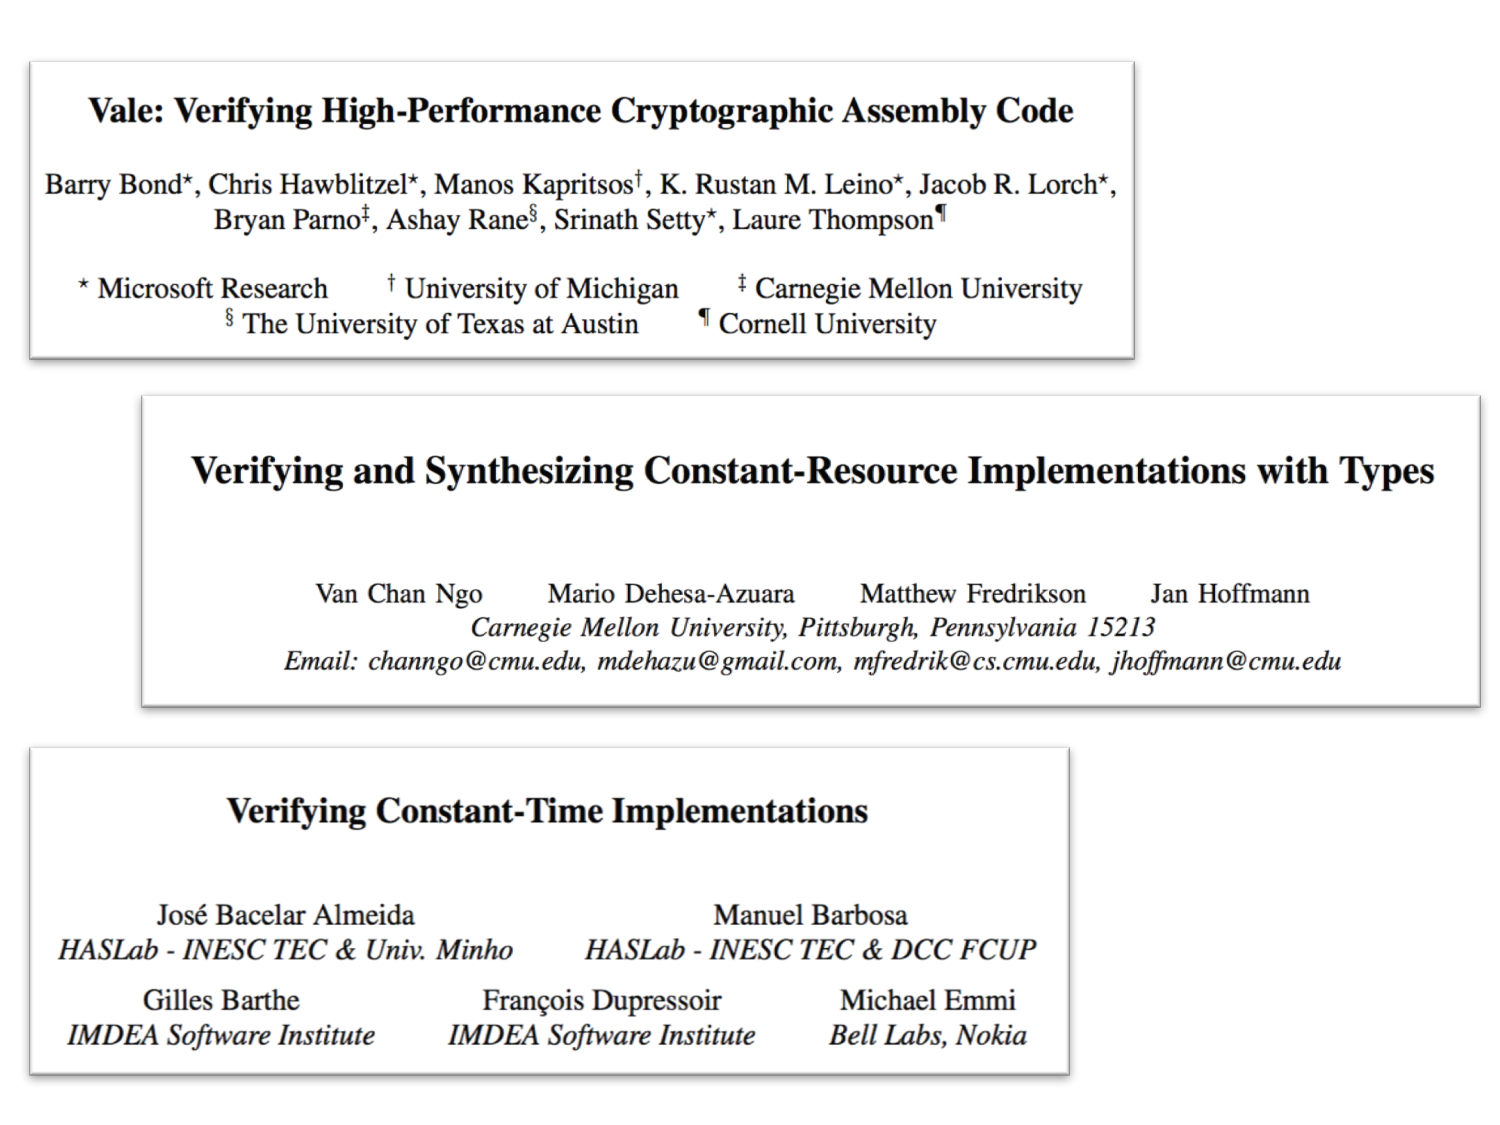
\includegraphics[width=\textwidth]{sidechan-papers.pdf}

\end{frame}

%%%%%%%%%%%%%%%%%%%%%%%%%%%%%%

\begin{frame}

\frametitle{Spectre \& Meltdown: Takeaways}

Security problems are numerous, can be subtle and challenging
\begin{itemize}
  \item Speculative execution isn't exactly new...
  \item Addressing it requires deep expertise, app-specific mitigations \\[2em]
\end{itemize}

\pause
This course will teach you how to deal with issues like this
\begin{itemize}
  \item Understand the essentials of many software security problems
  \item Evaluate potential solutions and their tradeoffs
  \item Implement strong defenses using principled techniques
  \item \textbf{Write code that isn't vulnerable in the first place}
\end{itemize}

\end{frame}

%%%%%%%%%%%%%%%%%%%%%%%%%%%%%%

\begin{frame}

\frametitle{Back to the course}

What is this course about?
\\[2em]

\centering


\includegraphics[width=0.4\textwidth]{whathappens.png}

\end{frame}

%%%%%%%%%%%%%%%%%%%%%%%%%%%%%%

\begin{frame}

\frametitle{This is not a course about encryption...}

\hspace*{-1.5em}
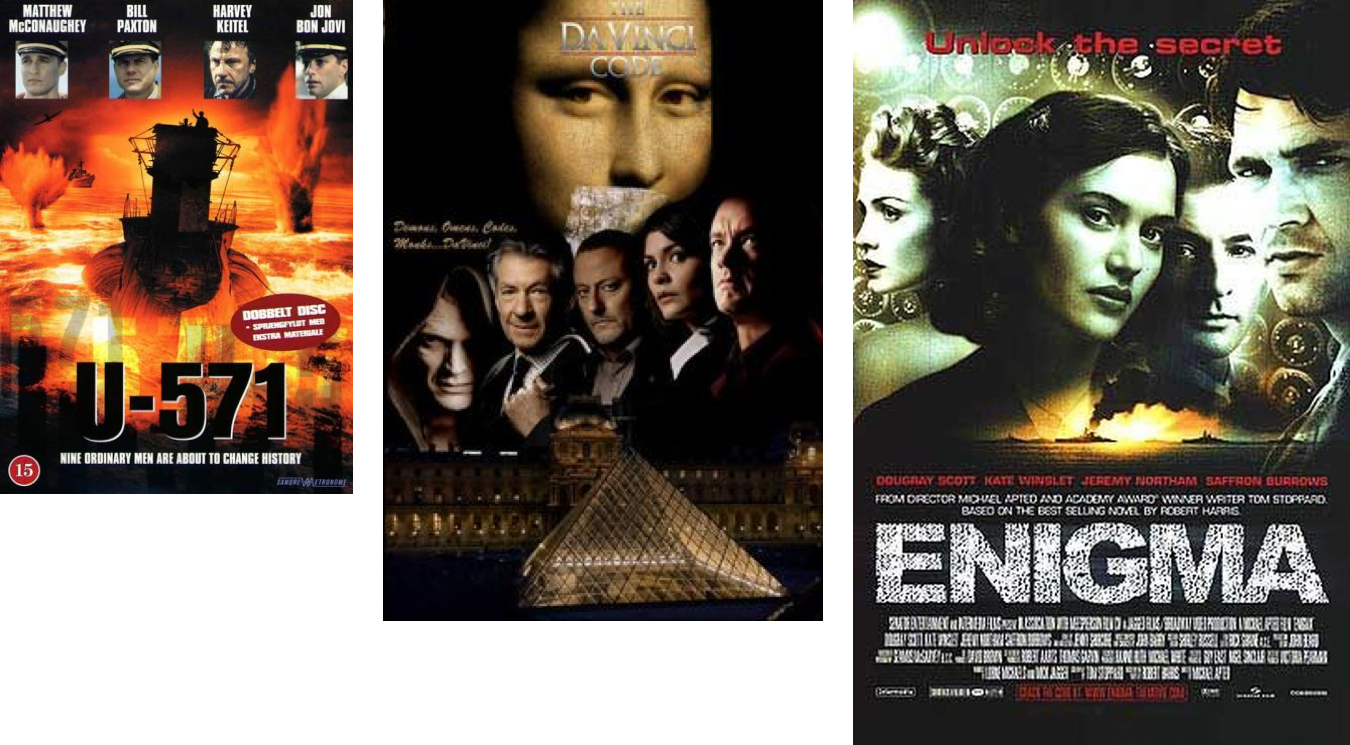
\includegraphics[width=1.1\textwidth]{crypto.png}

\end{frame}

%%%%%%%%%%%%%%%%%%%%%%%%%%%%%%

\begin{frame}

\frametitle{Not a course about hacking...}

\hspace*{-1.5em}
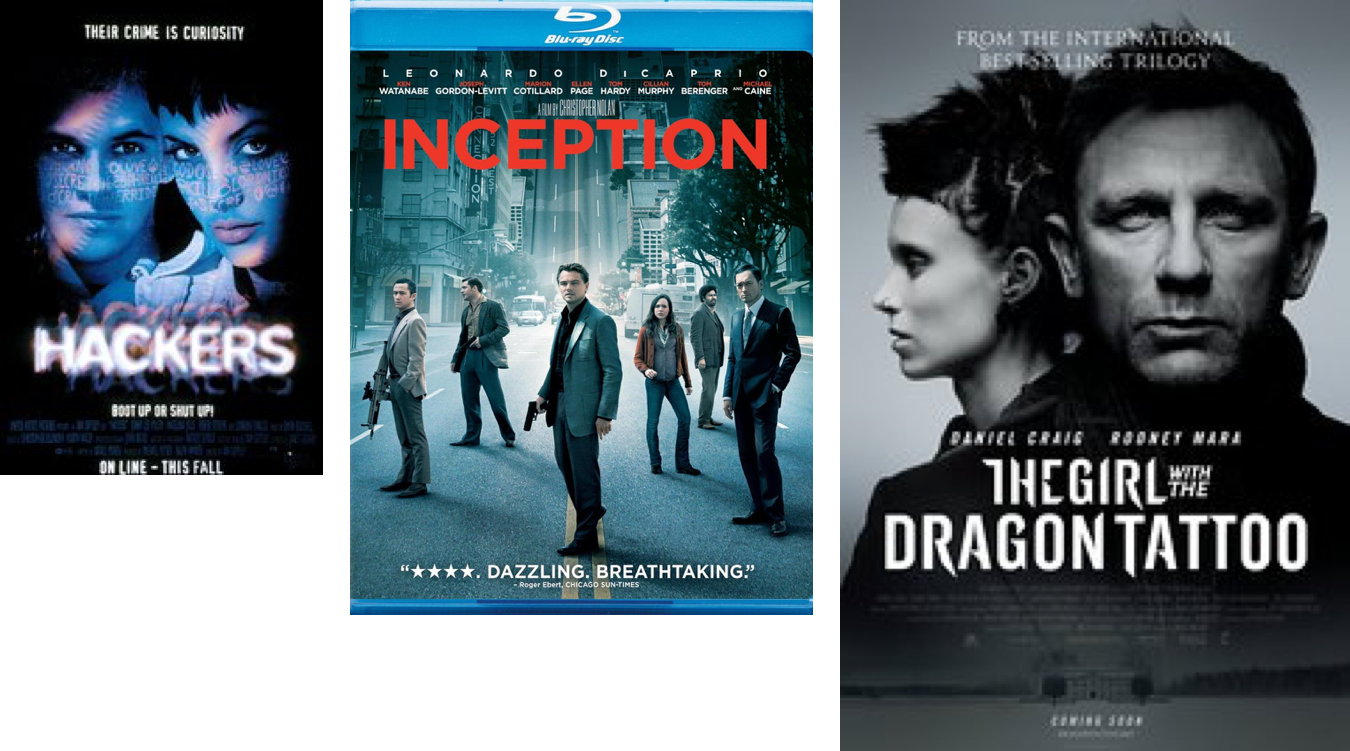
\includegraphics[width=1.1\textwidth]{hacking.png}

\end{frame}

%%%%%%%%%%%%%%%%%%%%%%%%%%%%%%

\begin{frame}

\frametitle{Not a course about social engineering...}

\hspace*{-1.5em}
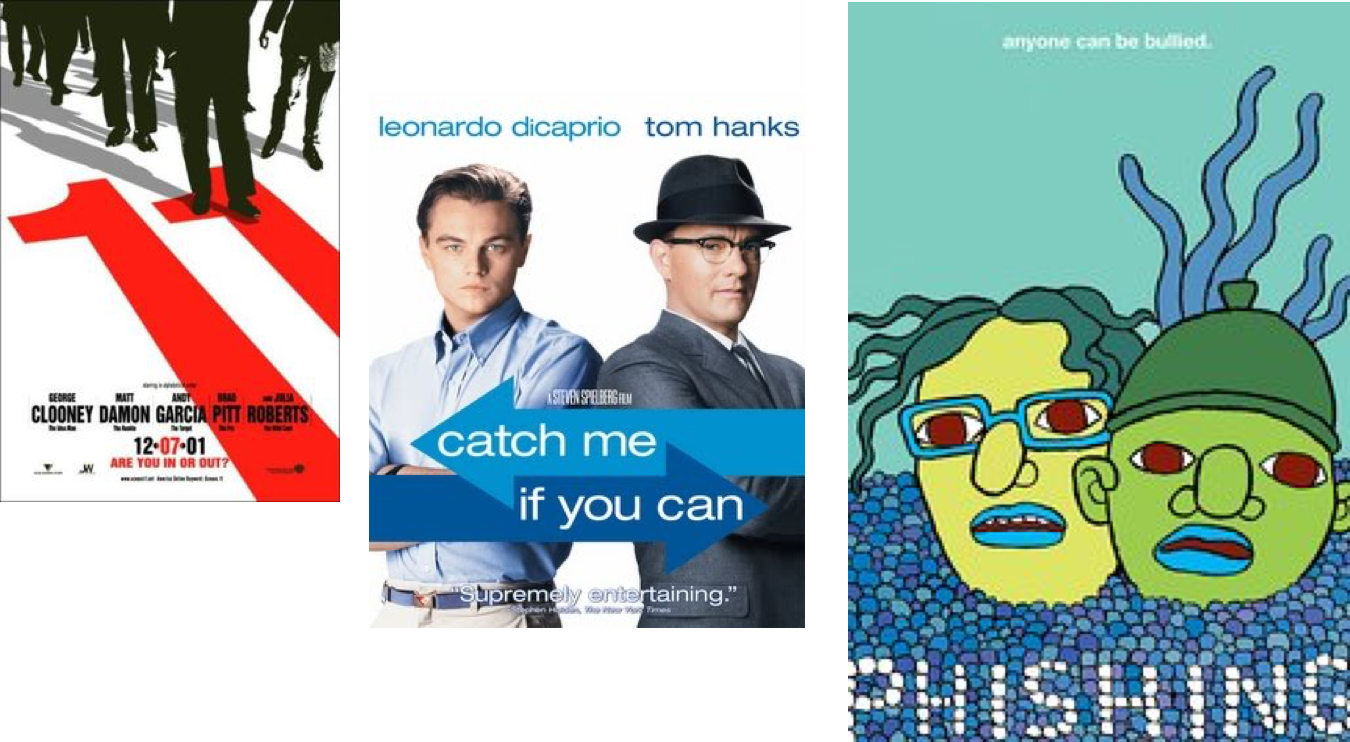
\includegraphics[width=1.1\textwidth]{social.png}

\end{frame}

%%%%%%%%%%%%%%%%%%%%%%%%%%%%%%

\begin{frame}

\frametitle{This course is about...}

\centering
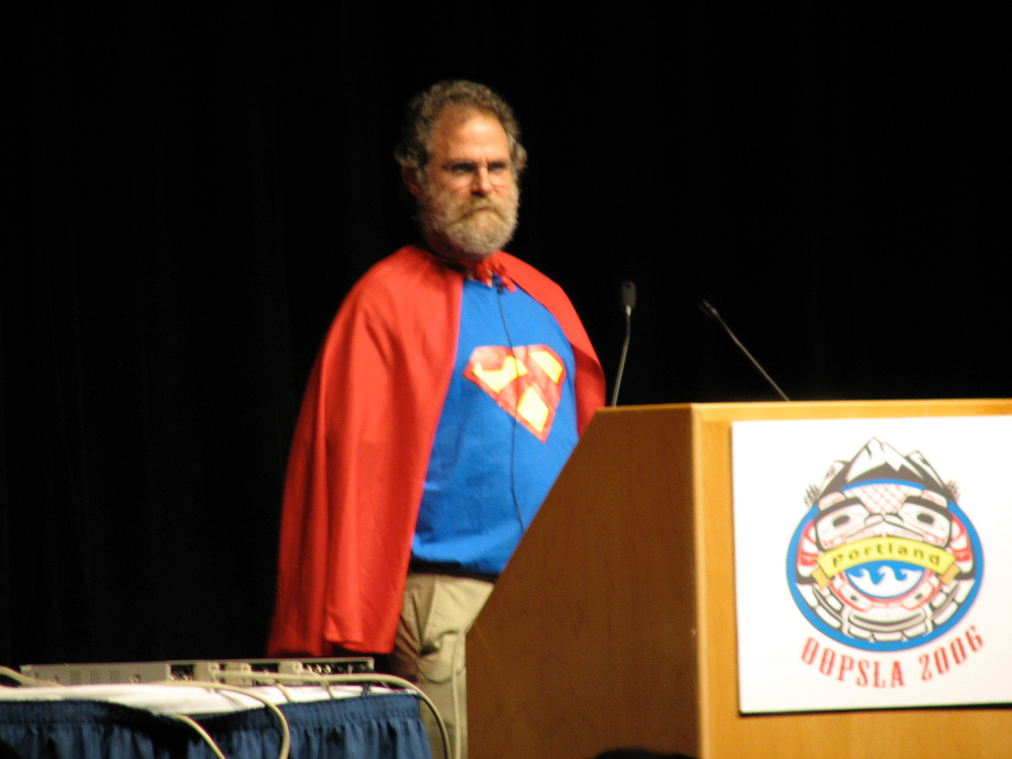
\includegraphics[width=0.8\textwidth]{wadler.png}

\vspace*{1em}
How logic and languages will save us (and make software secure)

\end{frame}

%%%%%%%%%%%%%%%%%%%%%%%%%%%%%%

\begin{frame}

\frametitle{Making software secure: desiderata}

Central theme: \emph{security \& correctness are often two sides of a coin}
\\[1em]

\pause
A way to specify software behaviors that are secure, i.e. \emph{policies} \pause
\begin{itemize}
  \item Who can see what data, and when?
  \item Under what circumstances can a program execute?
  \item ...and what do we expect of its outputs?
  \item How should information flow through a system? \\[1em]
\end{itemize}

\pause
A way to ensure that software adheres to policy, i.e. \emph{enforcement} \pause
\begin{itemize}
  \item With \textbf{convincing guarantees}, not ad-hoc arguments
  \item Often, without trusting developers or users
\end{itemize}

\end{frame}

%%%%%%%%%%%%%%%%%%%%%%%%%%%%%%

\begin{frame}

\frametitle{What logic \& languages gives us}

\textbf{Precise ways to write down policies} \pause
\begin{itemize}
  \item Types, contracts, functional specifications
  \item Devised for correctness, perfect for security as well \\[1em]
\end{itemize}

\pause
\textbf{Rigorous means of enforcement}
\begin{itemize}
  \item Type checking, formal verification for \emph{static} enforcement
  \item Runtime monitors, semantics-based instrumentation for \emph{dynamic} enforcement \\[1em]
\end{itemize}

\pause
\textbf{Convincing guarantees}: can \emph{prove} that enforcement ensures policy

\end{frame}

%%%%%%%%%%%%%%%%%%%%%%%%%%%%%%

\begin{frame}

\frametitle{Formality \& security}

Why is being formal such a big deal?
\\[1em]

\pause
Formal policies make assumptions and provisions explicit:
\begin{itemize}
  \item \textbf{Important}: these define the attacker's capabilities
  \item For security, formality means \emph{no surprises}! \\[1em]
\end{itemize}

\pause
(Useful) Formal guarantees can be proven if true, and refuted if not
\begin{itemize}
  \item ``Is my program secure'' is no longer a rhetorical question
  \item ...instead, a math problem
  \item If there's no proof, why should you trust it? \\[1em]
\end{itemize}

\pause
Formal techniques can often be automated

\end{frame}

%%%%%%%%%%%%%%%%%%%%%%%%%%%%%%

\begin{frame}

\frametitle{Formality \& security}

\large
\centering


\includegraphics[width=0.85\textwidth]{lazycat.jpg}

\end{frame}

%%%%%%%%%%%%%%%%%%%%%%%%%%%%%%

\begin{frame}

\frametitle{Formality \& security}

Why is being formal such a big deal?
\\[1em]

Formal policies make assumptions and provisions explicit:
\begin{itemize}
  \item \textbf{Important}: these define the attacker's capabilities
  \item For security, formality means \emph{no surprises}! \\[1em]
\end{itemize}

(Useful) Formal guarantees can be proven if true, and refuted if not
\begin{itemize}
  \item ``Is my program secure'' is no longer a rhetorical question
  \item ...instead, a math problem
  \item If there's no proof, why should you trust it? \\[1em]
\end{itemize}

Formal techniques can often be automated
\begin{itemize}
  \item While formal proof can be tedious, automation means less work
  \item Proof checkers mitigate human error, enable audit
\end{itemize}

\end{frame}

%%%%%%%%%%%%%%%%%%%%%%%%%%%%%%

\begin{frame}

\frametitle{What being formal doesn't give us}

Formalism isn't a panacea
\\[1em]

\pause
Proofs are relative to the formal definitions and assumptions in play
\begin{itemize}
  \item When these aren't realistic, neither are the guarantees
  \item See Cormac Herley's ``Unfalsifiability of security claims'' in \emph{PNAS} for a healthy dose of skepticism on this matter \\[1em]
\end{itemize}

\pause
Creativity, intuition, and good engineering are important for:
\begin{itemize}
  \item Devising and validating useful definitions
  \item Identifying the right threat model, assumptions
  \item Building robust and efficient implementations
\end{itemize}

\end{frame}

%%%%%%%%%%%%%%%%%%%%%%%%%%%%%%

\begin{frame}

\frametitle{Course topics}

Some of the topics that we will cover include:
\begin{itemize}
  \item Policy models: safety, information flow, statistical privacy
  \item Runtime policy enforcement, reference monitoring
  \item Security type systems
  \item Isolation (SFI, CFI, hardware protections)
  \item Trusted computing, authorization logic
  \item Web app security \& best practices
  \item Side channel vulnerabilities and defenses
  \item ...
\end{itemize}

\end{frame}

%%%%%%%%%%%%%%%%%%%%%%%%%%%%%%

\begin{frame}

\frametitle{Primary learning objectives}

After taking this course, you should:
\begin{enumerate}
  \pause\item Be able to identify, formalize, and implement useful security \& privacy policies
  \pause\item Understand the tradeoffs of different approaches to security \& privacy, and know how to reason about which one to use
  \pause\item Understand the role of key principles like least privilege, small trusted computing base, and complete mediation in formulating effective defenses
  \pause\item Be able to use formal proof and deductive systems to reason about the security of software systems
\end{enumerate}

\end{frame}

%%%%%%%%%%%%%%%%%%%%%%%%%%%%%%

\begin{frame}

\frametitle{Logistics}

\textbf{Website:} \url{https://15316-cmu.github.io}
\\[1em]

\textbf{Course staff contact:} Piazza

\textbf{Lecture}: Tuesdays \& Thursdays, 3:00-4:20 SH 214
\\[1em]

Matt Fredrikson
\begin{itemize}
\item Location: CIC 2126
\item Office Hours: Mondays 11am
\item Email: mfredrik@cs
\end{itemize}

\vspace*{1em}

Tianyu Li
\begin{itemize}
\item Office Hours: TBD
\item Email: tli2@andrew
\end{itemize}

\end{frame}

%%%%%%%%%%%%%%%%%%%%%%%%%%%%%%

\begin{frame}

\frametitle{Grading}

\begin{columns}
\begin{column}{0.45\textwidth}
Breakdown:
\begin{itemize}
\item 35\% labs
\item 30\% written homework
\item 30\% exams (15\% each, midterm and final)
\item 5\% participation
\end{itemize}
\end{column}

\begin{column}{0.55\textwidth}
Approximately 5 labs
\\[1em]

Written homework most weeks
\\[1em]

In-class exams, closed-book
\\[1em]

Participation:
\begin{itemize}
\item Come to lecture
\item Ask questions, give answers
\item Contribute to discussion
\item Be active and helpful on Piazza
\end{itemize}
\end{column}
\end{columns}

\end{frame}

%%%%%%%%%%%%%%%%%%%%%%%%%%%%%%

\begin{frame}

\frametitle{Written homework (30\% of grade)}

Written homeworks focus on theory and fundamental skills
\\[1em]

Grades are based on:
\begin{itemize}
\item Correctness of your answer
\item How you present your reasoning\\[1em]
\end{itemize}

Strive for \textbf{clarity \& conciseness}
\begin{itemize}
\item Show each step of your reasoning
\item State your assumptions
\item Answers without well-explained reasoning don't count!
\end{itemize}

\end{frame}

%%%%%%%%%%%%%%%%%%%%%%%%%%%%%%

\begin{frame}

\frametitle{Labs (35\% of grade)}

Extend C HTTP server to serve answers to data queries
\\[1em]

Incrementally add functionality while maintaining security
\\[1em]

Grades are based on:
\begin{itemize}
\item Whether you implemented correct functionality
\item Robustness to relevant attacks\\[1em]
\end{itemize}

Partial credit depending on:
\begin{itemize}
  \item How close your impl. is to the functional spec
  \item How many attacks your security measures prevent
\end{itemize}

\end{frame}

%%%%%%%%%%%%%%%%%%%%%%%%%%%%%%

\begin{frame}

\frametitle{What to do before Thursday}

\begin{enumerate}
  \item Make sure that you are enrolled in the Gradescope and Piazza sections for this course
  \item Bookmark the course webpage (\url{http://15316-cmu.github.io})
  \item Read the syllabus on the webpage carefully
  \item Contact the course staff (on Piazza!) if you have any questions
\end{enumerate}

\end{frame}

\end{document}
